\chapter{Evaluation}

The purpose of this chapter is to explain how the final iteration of the prototype was evaluated. The chapter will focus on the evaluation methods used, as well as representing data and discussing the results. The evaluation aimed towards concluding upon the final problem statement, and provide a better understanding about collaboration in groups.\\\\
The final test was conducted on a 4th grade at Skt. Annæ music elementary school. The goal of the test was to gather both quantative data as well as qualitative data. The qualitative test was a observation test, and the quantitative test was a Likert scale. These tests aim towards evaluating the prototype in correlation to the design requirements, as well as answering the final problem statement.

\section{Methods}
This section will describe the methods used in correlation to the methods presented in \autoref{chap:methods}. The section will present both the methods used to conduct the different tests, as well as which methods that has been used to analyse and conclude on the data. 

\subsection{Qualitative Test}
To get a better understanding of how the group collaborates; understanding how the group is using the prototype, and if they form some sort of group roles while using the prototype. To get a better view on the potential group roles, a non-participant test was conducted\ref{bjoernerBog}. Using a non-participant test will prevent the observers from being a part of the test and pottentially making the participants biased. Using this form of interview also creates a symbolisation of how the prototype would be used in a natural settings. A thing to keep in mind when conducting non-participant interviews, is that the data relies heavily on the observers interpretation of the events. Therefore it is important that the observer knows exactly what to look for. In this test, the observers relied heavily on the information gained from the analysis about group roles and collaboration\ref{bjoernerBog}.\\\\
(Insert data crunching method here :))

\subsection{Quantitative Test}
To test whether the test participants found the prototype collaborative or not, a Likert scale was used. The scale ranged from \textit{Disagree Strongly} to \textit{Agree Strongly}. The questions focused on statements which would give insight in how the test participant experienced the prototype in a collaborative manor. For all the questions on the Likert scale see appendix XX \ref{fig:likertScale}. The purpose of the Likert scale was for the participants to answer both positive as well as negative driven statements about differnet parts of collaboration i.e. if they felt that a person had more control than the others, or if they felt that they took part in the activities on the prototype.\\\\
Insert Methods about Likert scale data behandling.

\section{The Test}
As mentioned, the final test was conducted on a 4th grade on the Skt. Annæ music school. The total amount of testers were 25 students,  divided into 5 subgroups. Each group consisting of 5 participants took part in the activities on the prototype. Each group had a an approximate 10-13 minutes on the prototype, and 3-5 minutes filling out the Likert scale afterwards.

\subsection{The Setup}
The test was split up into 2 parts. The first part was where the students was executing the test while being observed. When the participants were lead into the room, they were first of, given a short introduction of how the prototype functions, and what the purpose of the prototype is. Afterwards, the participants were given the task to re-create the melody \textit{Mary Had a Little Lamb}, on the prototype. While playing the tune, the participants were being observed by 2 observers using the non-participant method\ref{bjoernerBog}. \\\\
When the participants completed the tasks, they were taken outside to complete a Likert scale about their collaboration using the prototype. 

Below might need to be sourced

\subsubsection*{Leader/Instructor}
The instructor role was the person that introduced the test participants to the test as well as introduced them to the tasks that the were to conduct. Furthermore, the instructor would answer any general questions, or questions regarding the execution of the test or the tasks. The same person also had a leader role and made sure that the test was conducted according to plan, and kept time of the test participant. This person would only introduce the prototype and the tasks, while staying out of the test as much as possible to avoid causing biased participants.

\subsubsection*{Observers}
The observers would sit in the back of the room while not talking or interacting with the test participants in any way. They used the non-participant method which means that they are not allowed to take any participation in the test. When the test participant entered the room, they were each given a sticker with a letter and a number on, for the observers to keep track of the different participants. The observers goal was to see if the test participant had patterns in a collaborative sense, while testing the prototype. They would observe factors such as group roles, if a natural leader would take place or everyone attempted to work together equally etc. Furthermore, the testers would observe which type of collaboration, if any, would take place. 

\subsubsection*{Likert Scale Conductor}
After the participants were finished interacting with the prototype, they would be led out of the room to take a Liker scale form. The conductor would hand out the papers and introduce the questions. While the participants being children, the conductor made sure to thoroughly explain each question and answer the participants question if they had any. Furthermore, the conductor would make sure that they did not affect the participants by presenting both positive and negative answers equally.

\subsubsection*{Runner}
The runner would help where help is needed, while the main task was to ready the next group of test participants while the other group were finishing up.\todo{Might be redundant}


\section{Results}
\begin{table}[H]
\centering
\caption{The results from the calculating the mean, variance and standard deviation on each question's responses (n=25).}
\label{table:questionsCalc}
\begin{tabular}{@{}cccclc@{}}
\toprule
\multicolumn{1}{l}{Question} & \multicolumn{1}{l}{Mean} & \multicolumn{1}{l}{Variance} & \multicolumn{1}{l}{Std} &  & \multicolumn{1}{l}{Cronbach alpha} \\ \midrule
1                            & 4.040                    & 0.8733                       & 0.934                   &  & 0.392                              \\
2                            & 4.080                    & 0.493                        & 0.702                   &  & 0.530                              \\
3                            & 4.160                    & 1.223                        & 1.106                   &  & 0.552                              \\
4                            & 3.480                    & 1.010                        & 1.004                   &  & 0.464                              \\
5                            & 3.680                    & 0.893                        & 0.945                   &  & 0.443                              \\
6                            & 3.680                    & 1.060                        & 1.029                   &  & 0.434                              \\
7                            & 3.040                    & 1.7067                       & 1.306                   &  & 0.807                              \\
8                            & 3.920                    & 1.326                        & 1.151                   &  & 0.412                              \\ \midrule
Overall                        & \multicolumn{1}{l}{}     & \multicolumn{1}{l}{}         & \multicolumn{1}{l}{}    &  & 0.5682                             \\ \bottomrule
\end{tabular}
\end{table}
to do\todo{to do}
% This file was created by matlab2tikz.
%
%The latest updates can be retrieved from
%  http://www.mathworks.com/matlabcentral/fileexchange/22022-matlab2tikz-matlab2tikz
%where you can also make suggestions and rate matlab2tikz.
%
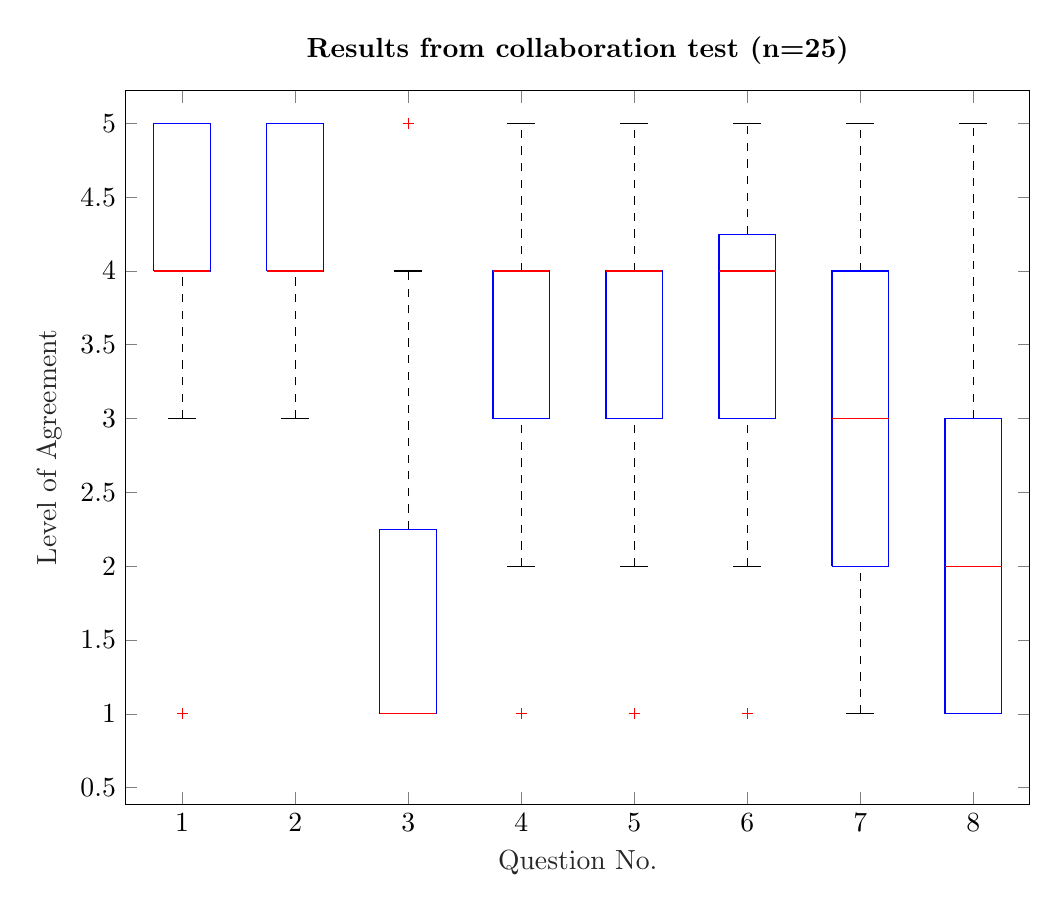
\begin{tikzpicture}

\begin{axis}[%
width=4.521in,
height=3.566in,
at={(0.758in,0.481in)},
scale only axis,
unbounded coords=jump,
xmin=0.5,
xmax=8.5,
xtick={1,2,3,4,5,6,7,8},
xlabel style={font=\color{white!15!black}},
xlabel={Question No.},
ymin=0.387875,
ymax=5.219625,
ylabel style={font=\color{white!15!black}},
ylabel={Level of Agreement},
axis background/.style={fill=white},
title style={font=\bfseries},
title={Results from collaboration test (n=25)},
legend style={legend cell align=left, align=left, draw=white!15!black}
]
\addplot [color=black, dashed, forget plot]
  table[row sep=crcr]{%
1	5\\
1	5\\
};
\addplot [color=black, dashed, forget plot]
  table[row sep=crcr]{%
2	5\\
2	5\\
};
\addplot [color=black, dashed, forget plot]
  table[row sep=crcr]{%
3	2.25\\
3	4\\
};
\addplot [color=black, dashed, forget plot]
  table[row sep=crcr]{%
4	4\\
4	5\\
};
\addplot [color=black, dashed, forget plot]
  table[row sep=crcr]{%
5	4\\
5	5\\
};
\addplot [color=black, dashed, forget plot]
  table[row sep=crcr]{%
6	4.25\\
6	5\\
};
\addplot [color=black, dashed, forget plot]
  table[row sep=crcr]{%
7	4\\
7	5\\
};
\addplot [color=black, dashed, forget plot]
  table[row sep=crcr]{%
8	3\\
8	5\\
};
\addplot [color=black, dashed, forget plot]
  table[row sep=crcr]{%
1	3\\
1	4\\
};
\addplot [color=black, dashed, forget plot]
  table[row sep=crcr]{%
2	3\\
2	4\\
};
\addplot [color=black, dashed, forget plot]
  table[row sep=crcr]{%
3	1\\
3	1\\
};
\addplot [color=black, dashed, forget plot]
  table[row sep=crcr]{%
4	2\\
4	3\\
};
\addplot [color=black, dashed, forget plot]
  table[row sep=crcr]{%
5	2\\
5	3\\
};
\addplot [color=black, dashed, forget plot]
  table[row sep=crcr]{%
6	2\\
6	3\\
};
\addplot [color=black, dashed, forget plot]
  table[row sep=crcr]{%
7	1\\
7	2\\
};
\addplot [color=black, dashed, forget plot]
  table[row sep=crcr]{%
8	1\\
8	1\\
};
\addplot [color=black, forget plot]
  table[row sep=crcr]{%
0.875	5\\
1.125	5\\
};
\addplot [color=black, forget plot]
  table[row sep=crcr]{%
1.875	5\\
2.125	5\\
};
\addplot [color=black, forget plot]
  table[row sep=crcr]{%
2.875	4\\
3.125	4\\
};
\addplot [color=black, forget plot]
  table[row sep=crcr]{%
3.875	5\\
4.125	5\\
};
\addplot [color=black, forget plot]
  table[row sep=crcr]{%
4.875	5\\
5.125	5\\
};
\addplot [color=black, forget plot]
  table[row sep=crcr]{%
5.875	5\\
6.125	5\\
};
\addplot [color=black, forget plot]
  table[row sep=crcr]{%
6.875	5\\
7.125	5\\
};
\addplot [color=black, forget plot]
  table[row sep=crcr]{%
7.875	5\\
8.125	5\\
};
\addplot [color=black, forget plot]
  table[row sep=crcr]{%
0.875	3\\
1.125	3\\
};
\addplot [color=black, forget plot]
  table[row sep=crcr]{%
1.875	3\\
2.125	3\\
};
\addplot [color=black, forget plot]
  table[row sep=crcr]{%
2.875	1\\
3.125	1\\
};
\addplot [color=black, forget plot]
  table[row sep=crcr]{%
3.875	2\\
4.125	2\\
};
\addplot [color=black, forget plot]
  table[row sep=crcr]{%
4.875	2\\
5.125	2\\
};
\addplot [color=black, forget plot]
  table[row sep=crcr]{%
5.875	2\\
6.125	2\\
};
\addplot [color=black, forget plot]
  table[row sep=crcr]{%
6.875	1\\
7.125	1\\
};
\addplot [color=black, forget plot]
  table[row sep=crcr]{%
7.875	1\\
8.125	1\\
};
\addplot [color=blue, forget plot]
  table[row sep=crcr]{%
0.75	4\\
0.75	5\\
1.25	5\\
1.25	4\\
0.75	4\\
};
\addplot [color=blue, forget plot]
  table[row sep=crcr]{%
1.75	4\\
1.75	5\\
2.25	5\\
2.25	4\\
1.75	4\\
};
\addplot [color=blue, forget plot]
  table[row sep=crcr]{%
2.75	1\\
2.75	2.25\\
3.25	2.25\\
3.25	1\\
2.75	1\\
};
\addplot [color=blue, forget plot]
  table[row sep=crcr]{%
3.75	3\\
3.75	4\\
4.25	4\\
4.25	3\\
3.75	3\\
};
\addplot [color=blue, forget plot]
  table[row sep=crcr]{%
4.75	3\\
4.75	4\\
5.25	4\\
5.25	3\\
4.75	3\\
};
\addplot [color=blue, forget plot]
  table[row sep=crcr]{%
5.75	3\\
5.75	4.25\\
6.25	4.25\\
6.25	3\\
5.75	3\\
};
\addplot [color=blue, forget plot]
  table[row sep=crcr]{%
6.75	2\\
6.75	4\\
7.25	4\\
7.25	2\\
6.75	2\\
};
\addplot [color=blue, forget plot]
  table[row sep=crcr]{%
7.75	1\\
7.75	3\\
8.25	3\\
8.25	1\\
7.75	1\\
};
\addplot [color=red, forget plot]
  table[row sep=crcr]{%
0.75	4\\
1.25	4\\
};
\addplot [color=red, forget plot]
  table[row sep=crcr]{%
1.75	4\\
2.25	4\\
};
\addplot [color=red, forget plot]
  table[row sep=crcr]{%
2.75	1\\
3.25	1\\
};
\addplot [color=red, forget plot]
  table[row sep=crcr]{%
3.75	4\\
4.25	4\\
};
\addplot [color=red, forget plot]
  table[row sep=crcr]{%
4.75	4\\
5.25	4\\
};
\addplot [color=red, forget plot]
  table[row sep=crcr]{%
5.75	4\\
6.25	4\\
};
\addplot [color=red, forget plot]
  table[row sep=crcr]{%
6.75	3\\
7.25	3\\
};
\addplot [color=red, forget plot]
  table[row sep=crcr]{%
7.75	2\\
8.25	2\\
};
\addplot [color=black, draw=none, mark=+, mark options={solid, red}, forget plot]
  table[row sep=crcr]{%
1	1\\
};
\addplot [color=black, draw=none, mark=+, mark options={solid, red}, forget plot]
  table[row sep=crcr]{%
nan	nan\\
};
\addplot [color=black, draw=none, mark=+, mark options={solid, red}, forget plot]
  table[row sep=crcr]{%
3	5\\
};
\addplot [color=black, draw=none, mark=+, mark options={solid, red}, forget plot]
  table[row sep=crcr]{%
4	1\\
};
\addplot [color=black, draw=none, mark=+, mark options={solid, red}, forget plot]
  table[row sep=crcr]{%
5	1\\
};
\addplot [color=black, draw=none, mark=+, mark options={solid, red}, forget plot]
  table[row sep=crcr]{%
6	1\\
};
\addplot [color=black, draw=none, mark=+, mark options={solid, red}, forget plot]
  table[row sep=crcr]{%
nan	nan\\
};
\addplot [color=black, draw=none, mark=+, mark options={solid, red}, forget plot]
  table[row sep=crcr]{%
nan	nan\\
};
\end{axis}
\end{tikzpicture}%

% This file was created by matlab2tikz.
%
%The latest updates can be retrieved from
%  http://www.mathworks.com/matlabcentral/fileexchange/22022-matlab2tikz-matlab2tikz
%where you can also make suggestions and rate matlab2tikz.
%
\definecolor{mycolor1}{rgb}{0.00000,0.44700,0.74100}%
\definecolor{mycolor2}{rgb}{0.85000,0.32500,0.09800}%
%
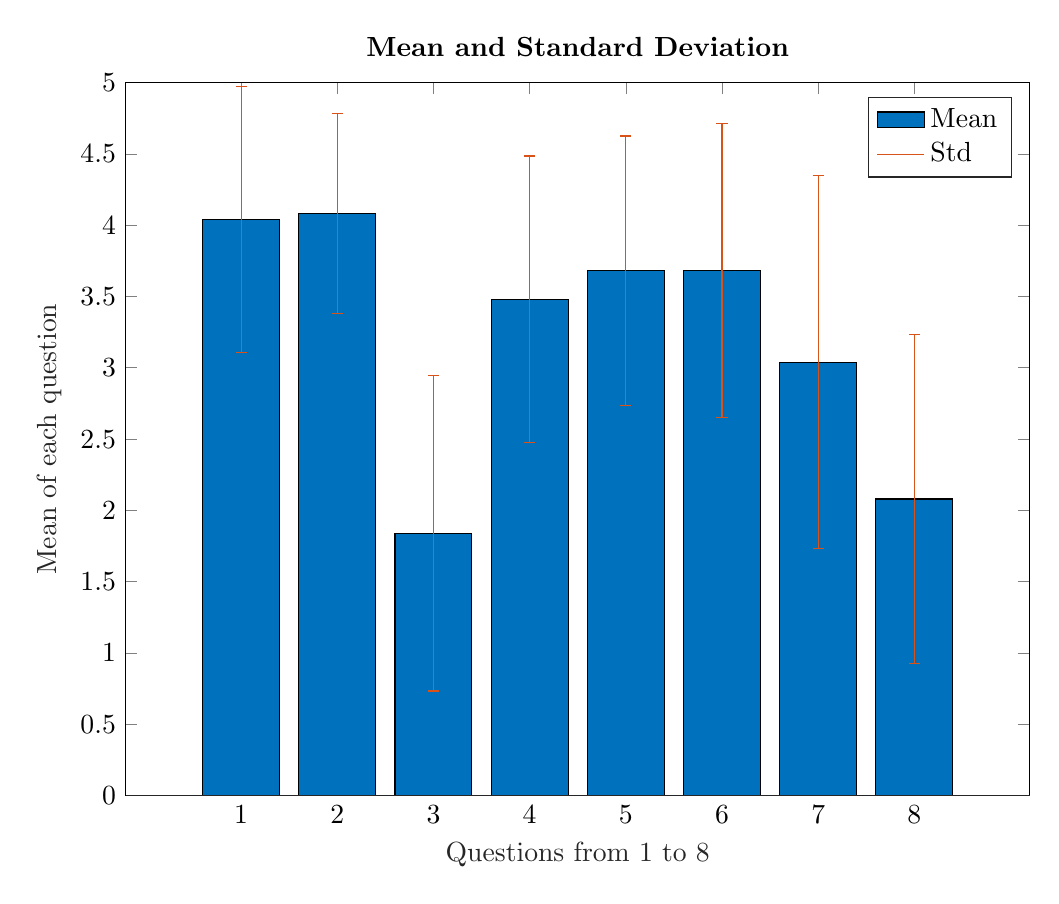
\begin{tikzpicture}

\begin{axis}[%
width=4.521in,
height=3.566in,
at={(0.758in,0.481in)},
scale only axis,
bar shift auto,
xmin=-0.2,
xmax=9.2,
xtick={1, 2, 3, 4, 5, 6, 7, 8},
xlabel style={font=\color{white!15!black}},
xlabel={Questions from 1 to 8},
ymin=0,
ymax=5,
ylabel style={font=\color{white!15!black}},
ylabel={Mean of each question},
axis background/.style={fill=white},
title style={font=\bfseries},
title={Mean and Standard Deviation},
legend style={legend cell align=left, align=left, draw=white!15!black}
]
\addplot[ybar, bar width=0.8, fill=mycolor1, draw=black, area legend] table[row sep=crcr] {%
1	4.04\\
2	4.08\\
3	1.84\\
4	3.48\\
5	3.68\\
6	3.68\\
7	3.04\\
8	2.08\\
};
\addplot[forget plot, color=white!15!black] table[row sep=crcr] {%
-0.2	0\\
9.2	0\\
};
\addlegendentry{Mean}

\addplot [color=mycolor2, draw=none]
 plot [error bars/.cd, y dir = both, y explicit]
 table[row sep=crcr, y error plus index=2, y error minus index=3]{%
1	4.04	0.934523051258413	0.934523051258413\\
2	4.08	0.702376916856849	0.702376916856849\\
3	1.84	1.1060440015358	1.1060440015358\\
4	3.48	1.00498756211209	1.00498756211209\\
5	3.68	0.945163125250522	0.945163125250522\\
6	3.68	1.0295630140987	1.0295630140987\\
7	3.04	1.30639452948436	1.30639452948436\\
8	2.08	1.15181016954473	1.15181016954473\\
};
\addlegendentry{Std}

\end{axis}
\end{tikzpicture}%


